% コンパイル:
% extractbb img/*.png
% platex soturon.tex
% pbibtex soturon
% platex soturon.tex
% dvipdfmx soturon

\documentclass{jsarticle}

\usepackage[dvipdfmx]{graphicx}
\usepackage{url}
\usepackage{slashbox}

%\usepackage{amsmath}
%\usepackage{txfonts}

\newcommand{\todayd}{\the\year--\the\month--\the\day}

\title{}
\date{\today}
%\affiliation{総合情報学科 メディア情報学コース}
%\supervisor{橋山智訓 准教授}
%\studentid{1310163}
\author{柴澤弘樹}
%\headtitle{平成28年度 総合情報学科 卒業論文中間発表}
\title{ぷよぷよの連鎖構築AIに関する研究}

\begin{document}
\maketitle

\part{序論} \setcounter{section}{0}
\section{背景}
\subsection{ゲームを取り巻く状況}
%遊びとコンピュータゲームの歴史
我々人類は、遊びと共に生きている。ホイジンガは「ホモ・ルーデンス」の中で、遊びが文化よりも古いものであると述べている\cite{homo}。現在遊ばれているコンピュータゲームもまた、遊びの一種といえる。藤田による調査\cite{huzita1,huzita2,huzita3}の中で、コンピュータゲームの一般への普及は、1980年代からであったことが述べられている。

%スマフォによる一般へのゲーム普及、e-sportの市場拡大
現在では、スマートフォンの普及と共にゲームプレイヤーがさらに増えている。ファミ通ゲーム白書2016\cite{famitu}により、アプリゲームを含むゲーム市場の拡大が示されている。さらには、eスポーツとして、ゲームでプレイヤー同士が競う大会も多く開催されている。大会やプロプレイヤーにはスポンサーがつき、世界規模の市場となっている\cite{e-sports}。これらの市場は、今後もますますの成長が期待されている。

%ネット対戦、AIは対戦相手として不足
このような背景の中で、遊びとしてのゲームはより身近なものになっている。様々なハードウェアでインターネットを介した協力、対戦プレイが可能となっており、遠く離れたプレイヤー同士で同じゲームをプレイすることも当然のこととなった。それによって、遊び相手として人間が一般的になり、AIを相手に長時間遊ぶゲームは限られたものとなってきている。ゲームAI技術は著しい発展を遂げてきたものの、遊び相手としては未だ向上の余地があるといえる。

%なぜAIである必要があるか? マッチング、練習、環境、対人への抵抗
インターネットを介した対人プレイにおいては、以下のような問題が挙げられる。
\begin{itemize}
\item 対応した環境の必要性
\item 十分なプレイ人口の必要性
\item プレイスキルを考慮したマッチング
\item 気兼ねない相手とはならない
\item 対人への抵抗感
\end{itemize}
以下、簡単に説明する。環境は、ゲームのハード、ソフト両面で整っている必要がある。インターネット環境の不足や、対応していないゲームではオンラインプレイが不可能となる。プレイ人口は、時間や発売からの経過日数などの影響を受ける。十分にプレイヤーが揃わなければ、マッチングができない。それに付随し、プレイスキルのバランスを考慮したマッチメイキングも必要となる。また相手が人間であるため、他プレイヤーを無視した勝手なふるまいが全くできない問題もある。ゲームを楽しんだり練習したりするため、あえて無駄な動きや非効率な行為をすることができないのである。心情的に、他人とゲームをプレイすることを忌避するプレイヤーも一定数いると考えられる。

以上の問題の通り、遊び相手としての人間が、必ずしも適しているとはいえない場面が存在する。このとき、ゲームAIは一つの解決策となる。そのため、プレイヤーに楽しさを提供する手法を研究し、遊び相手としてのAIを実現することに一定の意義があると考えられる。

\subsection{ゲームAIの現状}
%学術研究、コンペティション、強いAI
これまでのゲームAIの研究は、強いAIを目指したものだった。IEEE CIGをはじめとするAIコンペティション\cite{cig}や、人間との戦いによって強さが競われてきた。特に盤上ゲームでは、1997年のDeep Blue、2013のponannza、そして2015年のAlphaGo\cite{alphaGo}が、それぞれプロ棋士に初勝利を収めた。いまやAIは、人間と同等以上の強さをもつようになったと言える。つまり、AIの強さにおける研究は、一定の成果が得られたと言われるようになってきている。

%探索アルゴリズム、モンテカルロ法
強いAIを求めるこれまでの研究は、探索アルゴリズムの研究であったという見方ができる。完全情報ゲームの着手に評価を与え、最適解を探索する手法が様々提案されてきた。着手に対しどのような評価を与え、計算資源の中でいかに効率よく探索を行うかが問題だったのである。AlphGoでは、ディープニューラルネットワークによる評価と、モンテカルロ木探索によってそれらの問題を解決した。これらの手法は、AIの挙動がブラックボックスとなり、全容の理解が困難となる問題がある。その一方で汎用性が高く、様々に応用されている\cite{NE, monte}。完全情報ゲームに関しては十分な成果が得られたことから、今後の強さに関する研究は、不完全情報ゲームやGeneral Game Playing(GGP)へ移行してゆくと思われる。

%実際の恩恵、ユーザエクスペリエンスの向上を目的としたAI: miyake, yan_panorama
以上で述べた通り、これまでのゲームAIは、強さや性能を評価する場として、ゲームを用いていたにすぎない。人間プレイヤーのゲーム体験を向上させる域には達していないのである。しかし、強さが十分な領域に達したことで、今後はユーザエクスペリエンスを考慮したAIの研究が活発化してゆくといわれている\cite{miyake_genzai, ikeda}。YannakakisはゲームAI研究の分野を以下の10個に分類した\cite{yan_panorama}。
\begin{enumerate}
\item Non-player character(NPC) behavior learning
\item Search and planning
\item Player modeling
\item Games as AI benchmarks
\item Procedural content generation
\item Computational narrative
\item Believable agents
\item AI-assisted game design
\item Gneral game AI
\item AI in commercial games
\end{enumerate}
競争としてのみではなく、デザイナーやプレイヤーのことを考慮したAI研究がなされていることが分かる。ゲームの遊びや楽しさという側面が、今後ますます注目されてゆくことが予想される。


\section{目的}
%ぷよぷよ:e-sportsの実績、技術レベルの幅広さ、AIがダメダメ、探索問題としての難しさ
本研究では、人を楽しませる相手としてのAIを構成する手法を提案することを、最終目的とする。特にパズルゲームの「ぷよぷよ」を対象とし、その対戦AIを実装する。「ぷよぷよ」は、以下のような特徴をもつ。
\begin{itemize}
\item 長年にわたって親しまれているゲームである
\item 大会やe-sportsでの対戦実績がある
\item プレイヤースキルの幅が非常に広い
\item 対戦用AIの性能が不十分である
\item 探索問題として難しい題材である
\end{itemize}
「ぷよぷよ」は長年にわたって、対戦ゲームとして親しまれてきた。それにも関わらず、対戦相手としてのAIは未だ不十分である。また不完全情報ゲームであり、探索問題としても課題が残されている。以上の観点から、「ぷよぷよ」のAIが研究対象として意義をもつと考えられる。

%人を楽しませる対戦AI:連鎖、戦術
%連鎖構築が不十分:連鎖数、柔軟性、リアルタイム性
対戦における「ぷよぷよ」のプレイでは、連鎖構築や戦術が重要となる。上級者のプレイでは、十分な威力の連鎖を保持しつつ、相手を妨害したり、相手の妨害を阻止したりする戦術が用いられている。現状のAIでは、どちらも不十分である。この解決のためにはまず、より基本的な行為である、連鎖構築を満足に行えなければならない。対戦中での連鎖構築は、連鎖数、柔軟性、リアルタイム性の3点を満足することが大切であると考えられる。本研究では、この3点を満たす連鎖構築アルゴリズムを実現することを目的とする。

%解決すべき課題%難しさ、技術的課題:
%・スコア増加の長期的視点(NG:1手で消去, OK:3手で+1連鎖)
%・ランダム性とおじゃまによる先読みの難しさ
%・色の可換性、ツモ順によるパターン化の難しさ
%・累乗オーダでの計算量
%・リアルタイムの制約
「ぷよぷよ」の連鎖構築AIの実装にあたり、技術的課題は以下に挙げられる。
\begin{itemize}
\item 長期的視点に基づく探索
\item 不完全情報と妨害による先読みの難しさ
\item 完成形のパターン化の難しさ
\item 計算量の膨大さとリアルタイムの制約
\end{itemize}
大きな連鎖数を確保するためには、長期的視点に基づいてぷよの配置を決定する必要がある。同じ一手であっても、すぐに連鎖の威力を補強できる手よりも、数手先で連鎖数を増やすための布石とする手の方が有効である。このために先読みが必要になるが、配される手がランダムであること、リアルタイムに相手からの妨害があることを考慮すると、その可能性が膨大になる。さらにはそのランダム性から、連鎖の完成形をあらかじめ想定しておくことが、大きな手間となる。配された手から完成形を組みかえるような、柔軟性ある連鎖構築が望ましいのはそのためである。最後に、ぷよは操作をしなくとも自由落下するため、配置の決定に時間的制約がある。以上のような課題を解決する手法の研究が、本稿の目的である。

\section{本論文の構成}


\part{ぷよぷよについて} \setcounter{section}{0}
\section{発売タイトル}
最初の「ぷよぷよ」は、コンパイルより1991年に発売された。当初の「ぷよぷよ」には相殺がなく、1994年の「ぷよぷよ通」によってはじめて導入された。以降のシリーズの基本形はこの「ぷよぷよ通」であるとされ、AC(アーケード)版は現在でも大会で利用される。その後もシリーズは続いたものの売り上げは振るわず、コンパイルは経営破綻に陥った。

2003年の「ぷよぷよフィーバー」以降はセガによってぷよぷよが発売されている。2004年のWindows版「ぷよぷよフィーバー」で、初の公式ネット対戦が可能となった。対戦ルールは「クラシックルール」(実質的な「通」ルール)と「フィーバールール」が搭載されていた。
その後も家庭用ゲーム機や携帯ゲーム機に向けて複数のタイトルが発売されている。2014年には「ぷよぷよ」と同じく落ちものパズルゲームの「テトリス」を組み合わせた、「ぷよぷよテトリス」が発売された。「テトリス」と「ぷよぷよ」の対戦が可能となるなど、異色の作品であった。「ぷよぷよ」のルールは、主に「ぷよぷよ通」に準拠したものとなっている。最新作は2016年発売の「ぷよぷよクロニクル」で、インターネット対戦では「スキルバトル」「ぷよぷよ通」「ぷよぷよフィーバー」の3種類のルールがプレイできる。

その他、「ぷよぷよ!!クエスト」や「なぞぷよ」などの派生作品が、スマートフォン向けアプリなどで発売されている。これらはグラフィックやキャラクター、4つつながると消える点などは踏襲しているものの、対戦要素が無くシステムも異なるため、従来のぷよぷよシリーズとは別のゲームであるといえる。

シリーズ全体を通し、特に対戦において「ぷよぷよ通」が基準となっていることが読み取れる。これまでに様々な新ルール搭載のタイトルが発売されてきたものの、「通」のルールに置き換わるものは未だ現れていない。そこで本稿でも「ぷよぷよ通」のルールに準拠し、以下の「ぷよぷよ」に関する研究を進める。

\section{ルール} \label{rule}
本研究で扱う、「ぷよぷよ通」の基本的なルールと用語について説明する。

%フィールド、ツモ
%ツモ:ペア、ネクスト・ネクネク、4色、自分と相手は同一、
\subsection{フィールドとぷよ} \label{field_puyo}
\begin{figure}[hbt]
  \begin{center}
  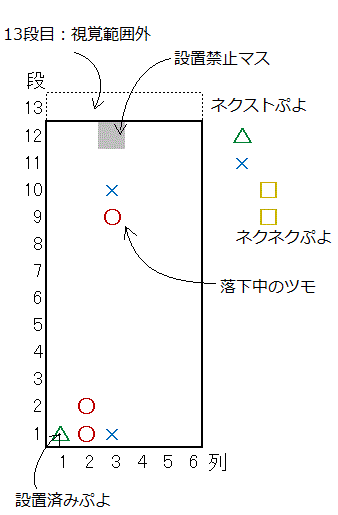
\includegraphics[height=10cm]{img/field.png}
  \caption{ぷよぷよのゲーム画面の概略} \label{fig:field}
\end{center}
\end{figure}

ぷよぷよのゲーム画面の概略図を、図\ref{fig:field}に示す。ぷよぷよのフィールドは、横6列$\times$縦12段が可視範囲である。以下、列数は左から数えたもの、段数は下から数えたものとする。配置するブロックは「ぷよ」と呼ばれる。3列目、12段目のマスにぷよを置くと窒息であり、負け(ばたんきゅ~)となる。また、実際にはフィールドに13段目があり、12段目にぷよがある状態で「回し」という操作技術を用いて、視覚範囲外へぷよを設置できる。13段目のぷよは可視できない状態で繋がったり消えたりすることはなく、12段目以下のぷよを消し、落下させることで連鎖に寄与する。

配石は2つのぷよがペアで現れ、これをツモという。ツモは落下中の物のほかに、次のツモ(ネクストぷよ)と次の次のツモ(ネクネクぷよ)が予め表示される。ぷよは複数の色から成り、対戦では最大4色が標準である。すなわち、4色のぷよが2つずつ現れることから、ツモは全16通りが存在する。対戦におけるツモ順は各プレイヤーで同一である。ツモの配色はランダムであり、表示される手数に上限があることから、配石に関する情報の不完全性が認められる。

ツモは3列目の13段目と12段目に現れ、自然に落下してゆく。落下中のツモは横移動と4方向回転ができるため、すでに埋まっていない限りは任意の列、あるいはそれと隣り合った列に配置できる。ぷよの設置の際は、下段に空白を認めない。下に空洞がある場合、それより上のぷよは全て下に落下する。よって、段差がある隣り合った2列に対しツモを横向きに置いた場合、片方のぷよが落下する。これを「ちぎる」という(図\ref{fig:tigiri}参照)。ツモの配置方法の選択は、異なる色の場合22通り、同色(ゾロ)の場合11通りとなる。
\begin{figure}[hbt]
  \begin{center}
  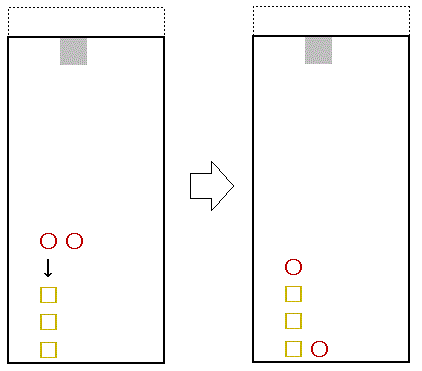
\includegraphics[height=7cm]{img/tigiri.png}
  \caption{「ちぎり」の発生の様子} \label{fig:tigiri}
\end{center}
\end{figure}

%消去、連鎖
\subsection{ぷよの消去と連鎖} \label{del_chain}
置かれた色ぷよは、上下左右に隣接したマスの同色ぷよと連結する。ここで色ぷよとは、後述の「おじゃまぷよ」ではない、ツモによって配されたぷよのことである。接続数が4以上となったぷよは、その時点ですべて消える。ぷよが消えたマスは空白となるが、その上部に別のぷよが存在する場合には、その落下により空白は埋められる。

\begin{figure}[hbt]
  \begin{center}
  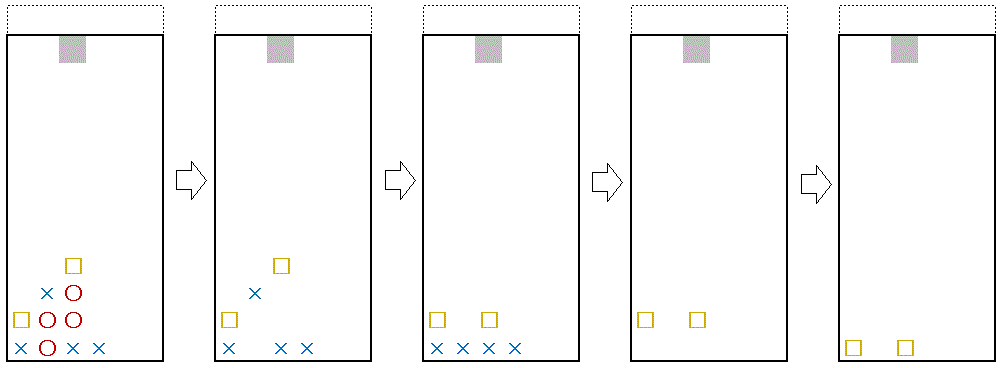
\includegraphics[height=6cm]{img/rensa.png}
  \caption{「連鎖」の発生の様子} \label{fig:rensa}
\end{center}
\end{figure}

ぷよが消えた後の落下により、さらに4つ以上接続されたぷよが現れた場合には、連続でぷよの消去が発生する(図\ref{fig:rensa}参照)。これを連鎖という。連続での消去がn回発生した際にはn連鎖となる。ぷよが消えるために最低4つを必要とし、フィールドは全78マスであるから、最大連鎖数は19連鎖である。また、連鎖を発動させるためにぷよを消去することを、「発火」という。

発火時には3列目12段目にもぷよを設置することができ、即座にはゲームオーバーとならない。ぷよの消去および連鎖の発生中には、新たなツモは発生せず、プレイヤーは操作ができない。連鎖がすべて終了した後に、操作可能となる。この時、3列目12段目にぷよが残っていると、その時点でゲームオーバーとなる。

%予告ぷよ、相殺、降るタイミング
%スコア
\subsection{スコアとおじゃまぷよ} \label{score_ojama}
ゲーム中には各プレイヤーのスコアが計算される。スコアは下キーによるぷよの落下操作時と、ぷよの消去および連鎖時、全消し時に増加し、1ゲーム中に減少することはない。落下操作時には、1マスにつき1点が加算される。全消しの際には2100点が加算される。n連鎖におけるスコアは、式\ref{fo:score}で算出できる。

\begin{eqnarray} \label{fo:score}
score & = & \sum_{i=1}^{n}(score_{i}) \nonumber \\
& = & \sum_{i=1}^{n}(delPuyo_{i} \times 10 \times bonus_{i})
\end{eqnarray}
ここで、$score$は発動した連鎖の合計スコア、$score_{i}$は$i$連鎖目のみのスコア、$delPuyo_{i}$は$i$連鎖目で消えたぷよの数、$bonus_{i}$は$i$連鎖目でのボーナス係数を表す。

ボーナスは、以下の3つのボーナスの総和で表される。
\begin{itemize}
\item 多色ボーナス:同時に消した色の数によるボーナス
\item 連結ボーナス:消したぷよの接続数によるボーナス
\item 連鎖ボーナス:連鎖数によるボーナス
\end{itemize}
それぞれのボーナス値を、表\ref{tab:color_bonus}、表\ref{tab:connect_bonus}、表\ref{tab:chain_bonus}に示す。ただし、ボーナスの総和が0の時には、値を1とする。

\begin{table}[htb]
\begin{center}
\caption{多色ボーナス} \label{tab:color_bonus}
\begin{tabular}{|l|r|r|r|r|} \hline
色数 & 1 & 2 & 3 & 4\\ \hline
ボーナス & 0 & 6 & 12 & 24\\ \hline
\end{tabular}
\end{center}
\end{table}

\begin{table}[htb]
\begin{center}
\caption{連結ボーナス} \label{tab:connect_bonus}
\begin{tabular}{|l|r|r|r|r|r|r|r|r|} \hline
連結数 & 4 & 5 & 6 & 7 & 8 & 9 & 10 & 11以上\\ \hline
ボーナス & 0 & 2 & 3 & 4 & 5 & 6 & 7 & 10\\ \hline
\end{tabular}
\end{center}
\end{table}

\begin{table}[htb]
\begin{center}
\caption{連鎖ボーナス} \label{tab:chain_bonus}
\begin{tabular}{|l|r|r|r|r|r|r|r|r|r|r|} \hline
連鎖数 & 1 & 2 & 3 & 4 & 5 & 6 & 7 & 8 & 9 & 10\\ \hline
ボーナス & 0 & 8 & 16 & 32 & 64 & 96 & 128 & 160 & 192 & 224\\ \hline
連鎖数 & 11 & 12 & 13 & 14 & 15 & 16 & 17 & 18 & 19 & -\\ \hline
ボーナス & 256 & 288 & 320 & 352 & 384 & 416 & 448 & 480 & 512 & -\\ \hline
\end{tabular}
\end{center}
\end{table}

対戦では、算出されたスコアに応じて、対戦相手におじゃまぷよが降る。スコア70点がおじゃまぷよ1つに相当する。70点以下は切り捨てられ、次回に持ち越される。対象となるスコアは、これまでにおじゃまぷよに換算されていないすべてのスコアである。つまり、落下操作や全消しで加算されたスコアは、次のぷよの消去時におじゃまぷよの換算に使われる。

おじゃまぷよは連鎖終了後、相手が落下中のツモを設置した時点(相手が次のツモを引く前)で降る。おじゃまぷよの落下列は都度ランダムに選ばれる。ただし一度に複数のおじゃまぷよが落ちる際には、偏りが少なくなるように落下列が選ばれる。例えば6個以下のおじゃまぷよが2段以上で降ることはなく、おじゃまぷよ6個はすべての列に1つずつ降る。なお、一度に降るおじゃまぷよの数は30個(5段)が上限であり、一度おじゃまぷよが降ると次の一手が配される。上限を超えておじゃまぷよが存在する場合、1手のツモを置いたのちに再度降ってくることとなる。

自分のフィールドにおじゃまぷよが降るまでには、相手の連鎖発火から連鎖が終了し、さらに自分が1手を置くまでの猶予がある。相手からおじゃまぷよが送られている間に自分の連鎖を発火すると、おじゃまぷよの相殺ができる。相殺の後に得点の高かったプレイヤーが、相手にスコアの差分だけおじゃまぷよを降らすことができる。相殺の途中で相手の連鎖が終了しており、かつ相殺し切れなかった場合には、自分の連鎖終了後即座におじゃまぷよが降って来る。
%タイムテーブル

\section{ぷよぷよの対戦}
\subsection{対戦文化と大会}
%95年:全日本ぷよマスターズ大会、ばよえ~んツアー
ぷよぷよの対戦は、ゲームの発売以降長い間にわたって続いてきた。公式大会の歴史は1995年にまでさかのぼることができ、コンパイル主催で「全日本ぷよマスターズ大会」や「ばよえ~んツアー」などが大々的に行われていた。

%100本先取
公式大会以外にも、有志によるゲームセンターやインターネット上での大会は数多く行われてきた。特に上位プレイヤーは、ゲームセンターのAC版「ぷよぷよ通」で強さを競い、全日本一位の座を目指した。試合形式は100本先取戦とされ、時として200試合近くに及ぶ対戦によって勝敗がつけられた。
試合は非公式であったものの、十分に試合回数を重ねることで、偶然性を排した強者のランキングがコミュニティの中で共有されていた。

%対戦文化:大会、e-sports
近年では、eスポーツ人気の高まりに伴い、ぷよぷよの大会にスポンサーがついたり、上位プレイヤーがテレビ番組に出演する機会が増えている。2016年の主な大会では、セガ公式「ぷよぷよ」最強プレイヤー決定戦\cite{sega}、第5回アーケード版ぷよぷよ通S級リーグ\cite{Skyuu}、A級リーグ\cite{Akyuu}、統一王座戦\cite{touituouza}、Red Bull 5G 2016\cite{5g}などが開催された。このように、ぷよぷよの発売以降現在でも、対戦ゲームとしての人気は高い。実用のプレイAIを実装するにあたっては、対戦を念頭に置くことが重要である。

%AIの到達点として、念頭におくべきこと
\subsection{対戦の基本的戦術} \label{senzyutu}
ぷよぷよは相殺のシステムにより、基本的に高い威力の連鎖を保持するプレイヤーが有利となる(\ref{score_ojama}参照)。お互いの連鎖を同時に発火した場合、スコアの高い連鎖が勝ち、一方的におじゃまぷよを送れるためである。連鎖の威力を上げるためには、同時に消すぷよの数や色の数を増やす、連鎖数を増やすといった方法がある。そのように連鎖を組むためには、ぷよを消さずにフィールドに積み上げる必要性がある。

%小連鎖によるつぶし
フィールドの多くがぷよで埋まっている状態では、少ないおじゃまぷよで残りのフィールドが埋まるために負けやすくなる。つまり、大連鎖を保持するプレイヤーを、小連鎖で倒すことが可能である。倒すまでには至らない場合でも、相手が連鎖を発火できない程度におじゃまぷよを送り、埋めてしまう(つぶし)ことが可能である。このように、単純に大連鎖のみの勝負とはならない奥深さがある。

%先打ち有利=>発火催促
さらに、片方のプレイヤーのみが大連鎖を発火した場面を考える。発火したプレイヤーの連鎖が進んでいる間も、もう片方のプレイヤーは操作が可能である。連鎖の終了までおじゃまぷよは降らないので、複数のツモを使って連鎖をさらに増やすことができる(伸ばし)。相手の連鎖が終了する前に後から伸ばした連鎖を発火すると、相手の連鎖を相殺し、おじゃまぷよを送り返すことすら可能である。このように、最初の発火時点で両者の連鎖威力が同等あるいは不利だったとしても、そのあとで状況を崩して有利にすることが可能である(後打ち有利)。

%催促合戦、凝視、組み換え(打つタイミング)
大連鎖を先に発火させるべく、相手の発火を促す戦術が成立する(催促)。大連鎖とは別に小連鎖を用意し、そちらを使って相手の発火を催促するのである。相殺できなければ潰されてしまい、発火しても不利な状況に陥る。このため、相手の小連鎖に対応するための小連鎖を、自分もまた用意する必要が出てくる。相手の状況を見て(凝視)、自分の連鎖を組む技術が重要になったのである。

以上で述べた通り、ぷよぷよの対戦にあたっては、連鎖数や威力だけでは語れない駆け引きが生じる。ここで述べた前提を基にして、様々な戦術や連鎖がこれまでに生まれてきた。これらを活用した強いAIを実装することもまた、ぷよぷよAIの重要な課題である。しかし、本稿ではそれを今後の課題とし、まずは大連鎖の構築に着目する。


\section{連鎖構築能力}
%対戦における実用的な連鎖とは何か? %なぜ連鎖数、柔軟性、リアルタイム性が必要か?
対戦において連鎖は、相手への攻撃手段でもあり、相手からの攻撃に対する防御手段でもある。そのため、連鎖を構築する能力は基本的かつ重要なものとなる。実戦の上で必要となる連鎖構築能力には、連鎖数、柔軟性、リアルタイム性が求められると考える。その内容を以下で説明する。

%連鎖数:フィールドの限界と効率
\subsection{連鎖の威力と連鎖数}
%スコア
連鎖を構築する目的の大部分が、大きなスコアを得るためである。なぜなら、スコアこそが相手に送れるおじゃまぷよの量を決定づけるからである。\ref{score}で述べた内容から、スコアを大きくするためには、ぷよの消える数や色を増やし、連鎖数を増やすことが有効であると分かる。しかし、フィールドに設置できるぷよの数には限りがあることに注意を要する。すなわち、フィールドを最大限効率よく使うために、同時消しの数をより増やすか、連鎖数をより増やすかを考えなければならない。

例えば、20個のぷよを全て消す場合を考える。4個消し5連鎖が合計4840点になるのに対し、2連鎖同時消し(1連鎖目で4個、2連鎖目で4色16個同時消し)では3240点となる(図\ref{fig:chain_score}参照)。つまり、同じぷよの数であれば、同時消しの数を増やすよりも、連鎖数を増やした方が、スコアが高くなるのである。これは連鎖ボーナス(表\ref{fig:chain_bonus})の上昇幅が大きく、さらに連鎖ごとに繰り返し点数が加算されることに起因する。よって限られたぷよ数で威力の高い連鎖を構築するためには、同時消しの数を減らし、連鎖数の効率を上げることが重要である。

%飽和連鎖量 %おじゃま、同時消し、形
組んでいる連鎖に同時消しの数が多かったり、フィールドにおじゃまぷよが存在していたりすると、必然的に連鎖数の上限が減ってしまう。このような観点から連鎖の効率を考える時、「飽和連鎖量」という概念を用いる。そのまま最大まで連鎖を伸ばしたとき、最終的な威力がどれほどとなるかを示す量である。現在保持している連鎖の量だけではなく、将来的にどれほど連鎖数を向上させることが可能かを考えることもまた、重要な能力である。そのような先読みによって、連鎖を完成させることよりもさらに伸ばすための布石を打つことを優先するような工夫ができ、飽和連鎖量を向上させることができるのである。

%柔軟性:ツモに合わせて完成形を変える %定型、不定形 %途中消し %合体、キーぷよ
\subsection{連鎖の柔軟性}
連鎖は、大きく定型連鎖と不定形連鎖に分けることができる。定型は、決まった連鎖形と名称が知られたものを指し、不定形は定型で無い連鎖を指す。それぞれの連鎖の例を、図\ref{fig:teikei}と図\ref{fig:huteikei}に示す。ぷよぷよでは配されるツモがランダムに決定されるため、それに合わせて連鎖を組む必要がある。定型連鎖では最終形に合わせてツモを配置してゆき、不定形連鎖ではツモに合わせて最終形を変えてゆく。どちらにしても、ツモに合わせて柔軟に配置を決定する必要がある。

%定型:色の可換性、おけない、混ぜ定型、途中けし
定型連鎖は完成形が定まってはいるものの、実際に組む時のぷよの配置が、固定化されたものであるとはいいがたい。まず、色の組み合わせに関して厳密に定めることが非現実である。例として3-1階段5連鎖を挙げると、図\ref{fig:kaidan5}に示したものは全て同じ形といえる。このように、同じ連鎖であってもその色の組み合わせは複数あり、完成形をただ一つに定めることができない。そして色の組み合わせは、ツモの落下順によって定まってゆくものである。一見して同じ形を組む場合であっても、ツモに応じた色の配置の変更が必要である。

その上、配置を固定化してしまうと、必ずしもツモを活かせないという欠点が表出する。図\ref{fig:kaidan_ng}で示したような例では、決められた連鎖形にするためにはツモを消すか捨てるかしかできない。しかし同じような場面でも、わずかに形を変えることで図\ref{fig:kaidan_ok}のようにツモを有効活用できる。たとえ定型連鎖であっても、ある程度形を変えられるような柔軟性を持たすことが有効である。ツモに合わせてぷよを配置する柔軟性があって初めて、余分なぷよを消して形を整えたり(\ref{fig:teikei_del})、定型連鎖をわずかに改変したり(図\ref{fig:teikei_combi})することが可能となる。このような配置の柔軟性をさらに顕著にしたものが、不定形連鎖である。

ツモを有効に活用するためには、配色に合わせて柔軟に形を選択し、ぷよを配置する能力が重要である。特に対戦では、相手からおじゃまぷよが送られてきた場合に、定型連鎖をそのまま維持することが困難となる。さらに相手に合わせた連鎖の用意などを見据えた場合、完成形を定めておくことは困難である。対戦で不定形連鎖が好まれるのは、ツモにあわせて連鎖形を変化させる柔軟性が大きな利点となるためである。


%リアルタイム性:早さによる有利・不利 %ちぎり、連鎖の速度(同時消しの強さ)
\subsection{リアルタイム性}
これまでに、連鎖を組む能力としてぷよの置き方に着目してきた。もう一つの重要な能力が、早さである。この早さには2種類があり、連鎖を組む早さと、連鎖自体の早さが考えられる。

連鎖を組む早さが勝負に影響することは明らかである。同じ威力の連鎖を組めるが、その早さが異なる2プレイヤーの対戦を考える。この場合、片方のプレイヤーが最大連鎖に到達した時点で、もう片方のプレイヤーは相手に劣る威力の連鎖しか保有できていない。当然、連鎖の打ち合いでは速度の遅いプレイヤーが負ける可能性の方が高くなる。威力のポテンシャルが同じでも、リアルタイムに進むゲームであるから、ある時点での保有連鎖量が異なることで有利不利が生じるのである。

ただし、\ref{senzyutu}で述べた通りに、後から連鎖を打つプレイヤーはさらに連鎖を伸ばす余地がある。相手の連鎖が終了するまでの時間、十分な速度で連鎖を組むことができれば、逆に有利な状況に立てる可能性がある。このように、連鎖を組む速度に応じてリアルタイムに戦況が変化する。早くツモをさばけるプレイヤーの方が、連鎖を増やすことや相手を妨害することにより多くのリソースを費やすことができるため、有利となる。

%連鎖を組む速度を向上させるためには、意思決定の高速化、操作の高速化、ちぎりを少なくするなどの方法がある。段差のある2列に対しぷよを横向きに設置すると、ぷよがちぎれて落下する。ちぎりによる落下速度は下キーの操作による移動よりも遅いため、頻繁に行うとタイムロスにつながる。

また連鎖数が増えると、アニメーションの描画が繰り返されるために発火から連鎖終了までの時間が長くなる。相手に対し即座におじゃまぷよを送りたい場合などでは、連鎖数を少なくする方が有効である。威力を犠牲にしてでも、同時消しや連鎖数の削減により機を逃さずに攻撃すべき局面が存在する。逆に相手が短時間の連鎖を仕掛けてきている時にも、将来的な連鎖数より現時点での短期的な連鎖の完成を目指すべきである。

連鎖構築能力としてのリアルタイム性には、連鎖を構築する早さを高めること、現時点と将来の盤面状況を判断して連鎖を組みかえることが求められる。対戦ではリアルタイム性が高いことを念頭に置き、時間の制約を意識することが肝要である。


\part{関連研究} \setcounter{section}{0}
\section{DQN}
why? how?
2015年
・事前知識、ルール不要
・従来手法を上回る性能
・プロゲーマーと同等以上?

パックマンは偶然による得点の取得が困難?


\section{ゲームと楽しさ}
\section{楽しさに関するゲームAI}
%実用レベルの対戦相手に向けて:手加減、自然さ、人間の模倣、プレイヤーモデル
%ikeda
DDA
player modeling: yannnakakis
mario

\section{ぷよぷよAI}
\section{その他のパズルゲームAI}
how?

\part{DQNによる学習} \setcounter{section}{0}
\section{とこぷよ}
\section{対戦}

\part{連鎖ポテンシャル法の改良} \setcounter{section}{0}
\section{探索深さの変更}
\section{全探索}
\section{途中での消去}
\section{ツモ選択と置き方選択の区別}

\part{人間の知識適用} \setcounter{section}{0}
\section{連鎖構築知識の抽出}
\section{ルール化と実装}
\section{結果と考察}

\part{結論} \setcounter{section}{0}
\section{研究成果}
\section{今後の課題}

%参考文献
\bibliographystyle{jplain}
\bibliography{ref}

\end{document}

